%%%%%%%%%%%%%%%%%%%%%%%%%%%%%%%%%%%%%%%%%%%%%%%%%%%%%%%%%%%%%%%%%%%
\section{Introduction}\label{sec:methodo_intro}

À cause des pressions énergétiques et économiques, les plateformes de calculs haute performance doivent être repensées. De nouvelles architectures optimisées pour certaines applications devront être utilisées rendues possibles grâce au protocole \verb=Gen-Z=. En l'absence de méthode de caractérisation fine de la performance des codes, ces architectures innovantes sont potentiellement condamnées puisque peu d'experts savent les valoriser. Cependant, ces nouvelles architectures, très différentes de celles utilisées aujourd'hui (x86, GPU), doivent être caractérisées pour prédire le gain de performance pour les applications. Pour pouvoir profiter de ces technologies et les utiliser de façon optimale, nous avons présenté dans le chapitre précédent une suite de logiciels de caractérisation et d'analyse de performance. L'objectif de ce chapitre est de présenter une méthodologie adaptée,  permettant de réaliser cette caractérisation ainsi que le portage des applications sur ces nouveaux accélérateurs.



\subsection{Motivation}
%%%%%%%%%%%%%%%%%%%%%%%%%%%%%%%%%%%%%%%%%%%%%%%

    La \autoref{sec:edl_hpc_hetero} aborde les principaux avantages de l'utilisation de plateformes hétérogènes dans les centres de calculs. Pour motiver le développement de la méthodologie présentée dans ce chapitre, nous discutons des principaux challenges à relever pour pouvoir en profiter.
       
    \subsubsection{L'hétérogénéité des supercalculateurs modernes}\label{sec:methodo_intro_hetero}
    %%%%%%%%%%%%%%%%%%%%%%%%%%%%%%%%%%%%%%%%%%%%%%%
        
        Depuis 2010, l'utilisation d'un accélérateur pour assister le travail des processeurs est de plus en plus répandue. La \autoref{pic:methodo_top500_accelerator} montre l'évolution du nombre de systèmes utilisant au moins un accélérateur par serveur. En 2019, près d'un tiers des plateformes utilisent un accélérateur (145/500) et nous remarquons une forte progression ces deux dernières années.  Cette évolution peut être en partie expliquée par l'utilisation extensive de GPU pour les applications d'intelligence artificielle dont l'entraînement des modèles est particulièrement adapté aux architectures des GPU.
        
        \begin{figure}
            \center
            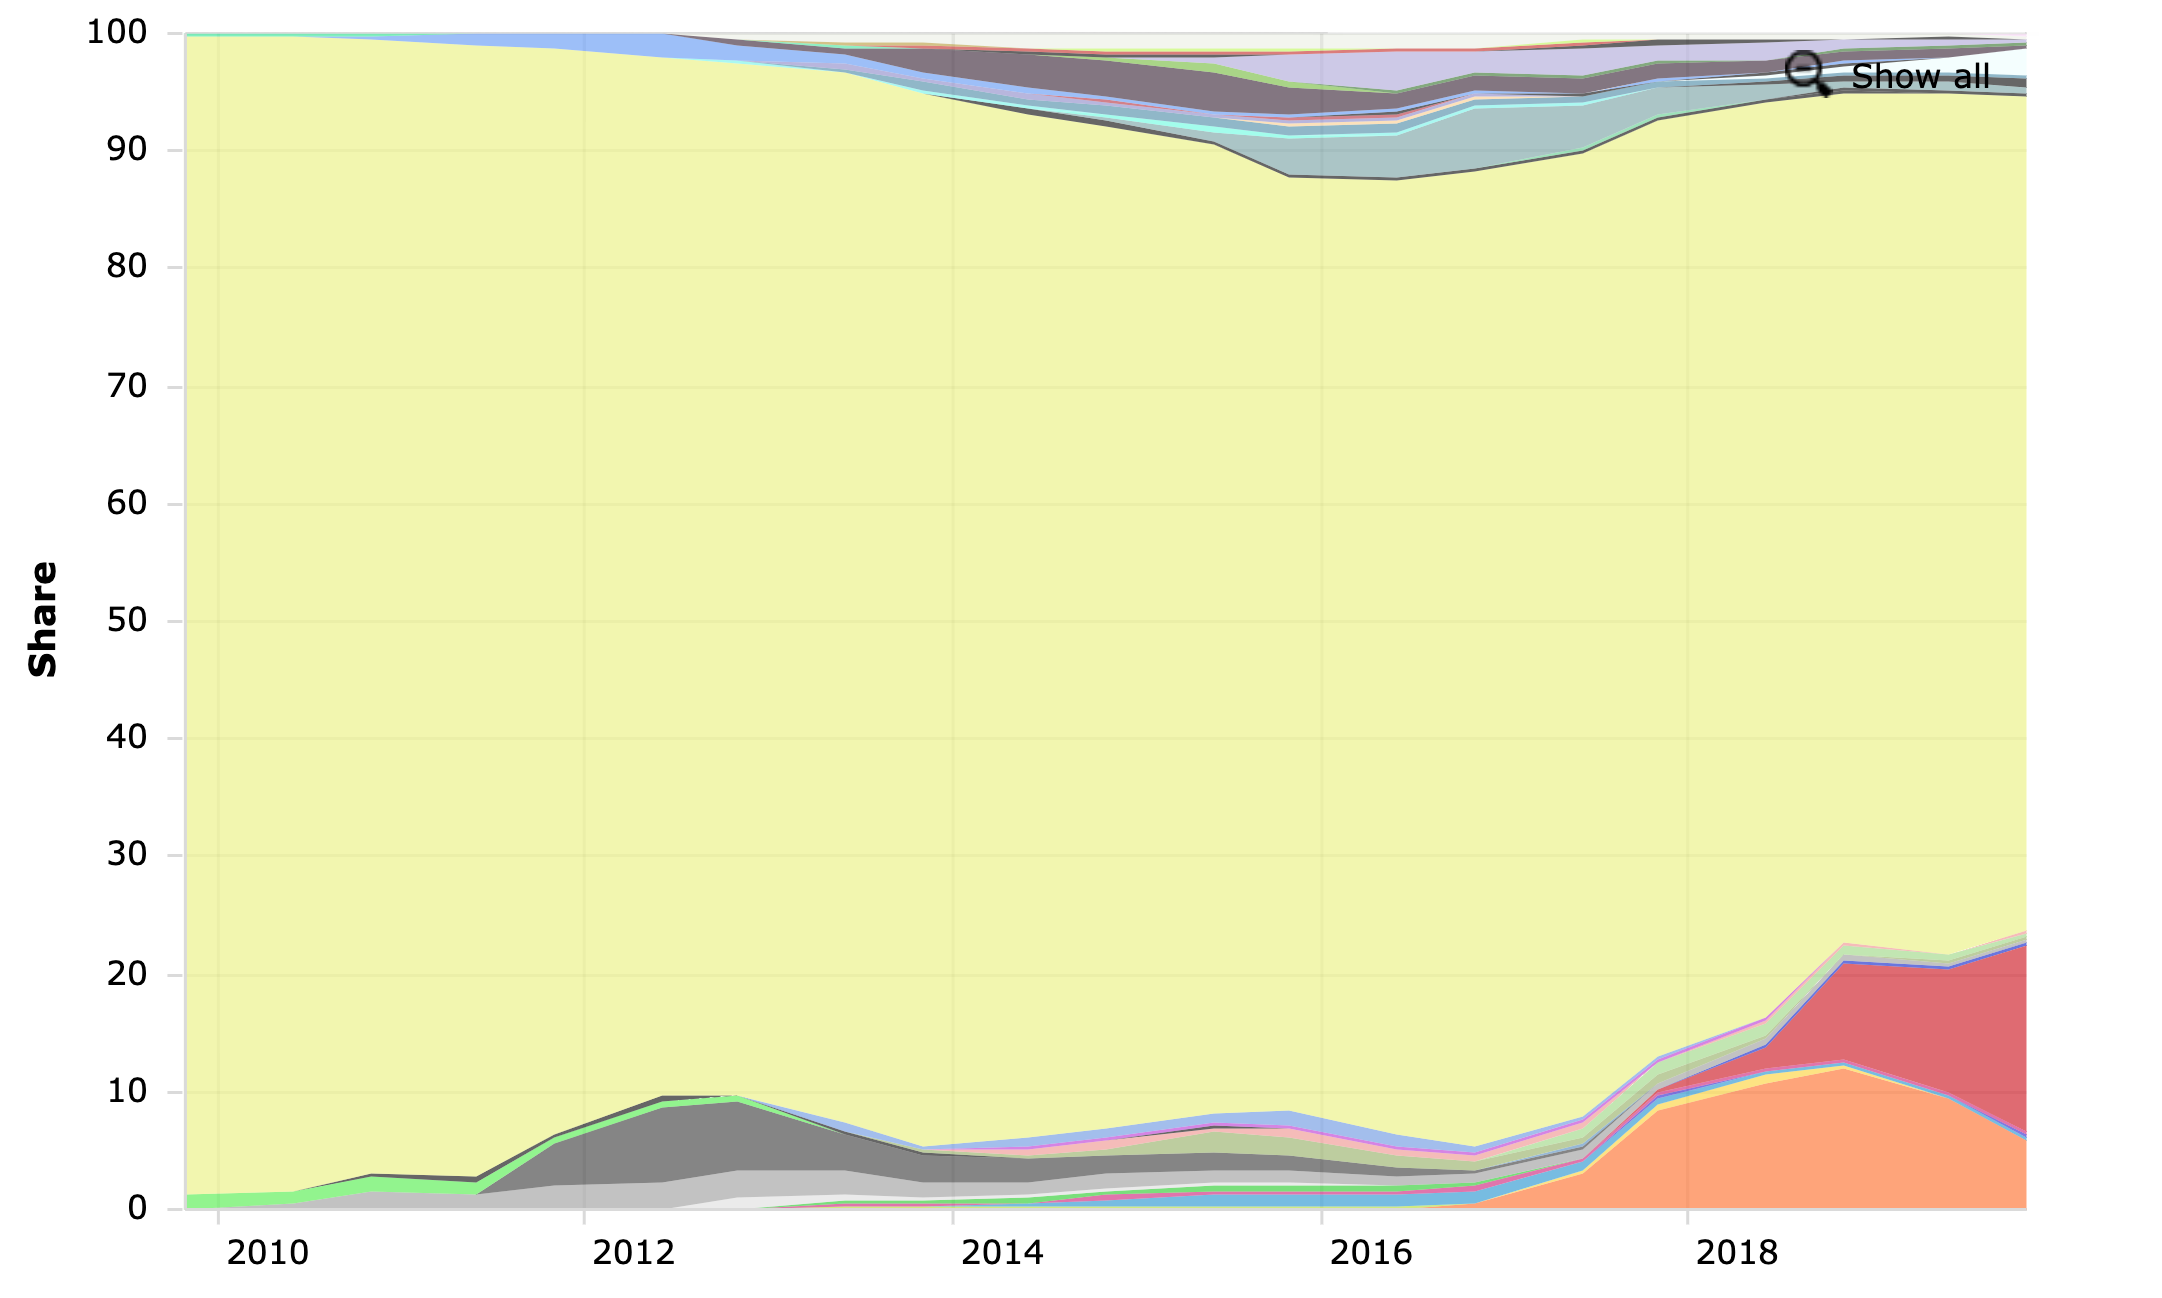
\includegraphics[width=12cm]{images/methodo_top500_accelerator.png}
            \caption{\label{pic:methodo_top500_accelerator} Évolution du nombre de supercalculateurs utilisant un accélérateur\protect\footnotemark. La partie en jaune représente les systèmes n'en utilisant pas.}
        \end{figure}
        \footnotetext{source : TOP500 - \url{https://www.top500.org/statistics/overtime} }
        
        
        Bien que cette évolution semble se confirmer avec la publication du dernier classement du TOP500 en novembre 2019, il est important de s'intéresser à la nature des accélérateurs utilisés.
        En 2018, plus de 96\% des processeurs des supercalculateurs du Top500 ont une architecture x86 et la majorité d'entre eux (91\%) proviennent du constructeur Intel. Seulement 28\% des 500 calculateurs sont associés à des accélérateurs dont 92\% sont des GPU provenant du constructeur NVIDIA. Bien que les systèmes profitent de l'hétérogénéité des matériels, il est intéressant de remarquer que leur composition est en réalité très similaire: un processeur Intel x86 associé à un GPU NVIDIA.
        
        En 2019, un seul type d'accélérateur est utilisé (GPU) et n'est utilisé que pour un sous-ensemble d'applications. Pour la construction de plateformes Exascale optimisée pour la majorité des applications, il faut suivre le même raisonnement. Cependant, la particularité des applications d'apprentissage par machine est leur profil uniforme. La majorité des applications de HPC sont composées de plusieurs tâches pouvant avoir des besoins très différents. Pour que ces applications puissent aussi profiter de l'hétérogénéité, les plateformes doivent posséder différents types d'accélérateurs pour y exécuter les noyaux de calculs d'une application. L'utilisation de plusieurs accélérateurs nécessite alors de devoir transférer les données pour poursuivre le traitement. Le déplacement des données
        
    
    \subsubsection{L'opportunité Gen-Z}
    %%%%%%%%%%%%%%%%%%%%%%%%%%%%%%%%%%%%%%%%%%%%%%%
       
        Avec le développement de \verb=Gen-Z=, le déplacement de données et la difficulté d'agrégation de différents matériels seront réduits. Ce protocole, présenté dans le chapitre \ref{sec:edl_hpc}, va révolutionner le monde de l'informatique comme peu de technologies auparavant. Entre tous les bénéfices apportés par ce protocole, la faculté de rendre facile l'hétérogénéité dans les supercalculateurs est sans doute la plus importante. L'hétérogénéité sera à la fois entre des accélérateurs spécialisés pour différents noyaux d'une application, mais aussi dans les architectures elles-mêmes permettant de mixer et d'adapter chaque coprocesseur. 
        
        Si certains constructeurs et utilisateurs continuent d'utiliser la même stratégie d'ajouter des serveurs \textit{standards} comme jusqu'à aujourd'hui, ils seront dépassés par ceux ayant commencé à investir ces nouvelles technologies plusieurs années avant eux. Il est donc crucial de s'y préparer en ayant la bonne méthodologie et les bons outils pour pouvoir en profiter. L'accès à des plateformes Exascale et à ces nouvelles architectures va aussi ouvrir de nouveaux marchés, inaccessible aujourd'hui à cause de plusieurs contraintes: le prix, la bande passante nécessaire, la sécurité ou encore la consommation électrique. 
        
        Les gains de performance ne viendront pas seulement par l'utilisation d'accélérateurs puissants, mais de leur diversité et de la capacité des programmeurs de bien les utiliser. Pour une même application, plusieurs accélérateurs spécialisés seront souvent nécessaires. On peut en imaginer certains adaptés à la lecture et à la décompression du jeu de données. Une fois réalisés, des accélérateurs spécialisés dans le calcul demandé pourront être utilisés (ASIC, FGPA ou DSP). Enfin pour la visualisation des données, des GPU seront alors nécessaires. L'hétérogénéité est à la fois un challenge majeur des plateformes Exascale, mais aussi une grande opportunité. 
        
    
\subsection{Contributions}
%%%%%%%%%%%%%%%%%%%%%%%%%%%%%%%%%%%%%%%%%%%%%%%

    Pour pouvoir profiter de l'hétérogénéité des accélérateurs, un travail préalable est nécessaire. Le premier est de caractériser ces plateformes, pour déterminer leurs forces, leurs faiblesses et leur efficacité pour un type d'application. Un second travail consiste à étudier l'application et à déterminer les besoins des noyaux de calculs la composant.
    
    
    \subsubsection{Délimitation de l'analyse}
    %%%%%%%%%%%%%%%%%%%%%%%%%%%%%%%%%%%%%%%%%%%%%%%

        Ces deux tâches peuvent être réalisées à plusieurs niveaux, que ce soit à l'échelle d'une grappe de serveurs, ou du processeur lui-même. Pour que le travail soit réalisable durant la thèse, nous avons délimité un certain cadre pour appliquer notre méthodologie (voir \autoref{pic_analyse}).
        
         \begin{figure}[h!]
            \center
            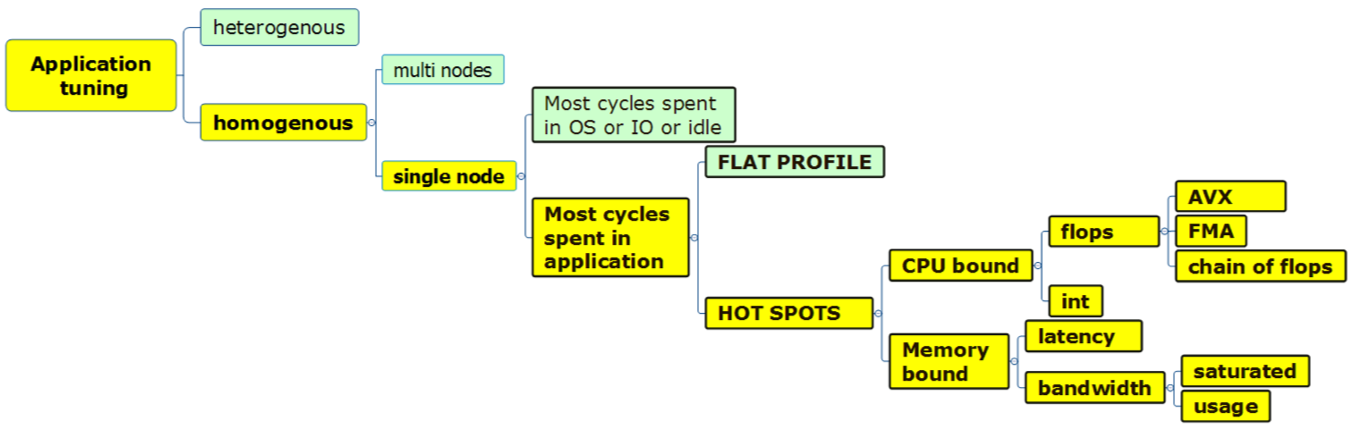
\includegraphics[width=14cm]{images/analyse.png}
            \caption{\label{pic_analyse} Délimitation de l'analyse proposée.}
        \end{figure}
        
        Les applications que nous ciblons dans notre analyse sont des codes dont la majorité du temps d'exécution se déroule seulement dans quelques pourcentages des lignes de codes. Nous appelons ces zones des points chauds, \textit{hot spots} ou encore \textit{kernels}. Une application possédant des hot spots est un gage d'un potentiel d'amélioration des performances. La performance de ces noyaux de calculs doit être limité par la mémoire ou par la puissance de calculs.
        La méthodologie s'intéresse à la performance de l'application sur un noeud de calculs. Les problèmes de performance liés à l'exécution sur plusieurs serveurs ne sont pas abordés bien que nous recommandions l'utilisation d'outils tels que \verb=Paraver=, \verb=Extrae= ou \verb=Tau= pour les détecter. Notre analyse se concentre sur la performance d'un noeud. Les applications dont la performance est limitée par  celle du système de stockage, du réseau ou du système d'exploitation ne sont pas la priorité de la méthodologie présentée (bien qu'ils puissent être décelés).
        
        Du fait de la complexité des architectures, le travail de portage et d'optimisation peut être très difficile. Ainsi, notre démarche s'adresse aux programmeurs ayant de solides connaissances des microarchitectures. Pour améliorer la précision de l'analyse et des outils ainsi que d'appliquer des transformations de code il est préférable d'avoir accès au code source. 
    
        
    \subsubsection{Organisation du chapitre}
    %%%%%%%%%%%%%%%%%%%%%%%%%%%%%%%%%%%%%%%%%%%%%%%
    
        Dans ce chapitre, nous présentons une méthodologie simple en 5 étapes permettant aux utilisateurs de modéliser les performances de leur code, de les projeter sur de nouvelles architectures et de les optimiser (voir \autoref{pic:methodologie_step_2}). Nous proposons un modèle de performance simple basé sur les caractéristiques du sous-système mémoire. L'objectif est de créer pour chaque \textit{hot spot} un modèle de ses performances dans le but de projeter ses performances sur d'autres architectures, mais aussi de valider ses performances. Nous cherchons à prouver la bonne utilisation ou non du système mémoire, ressource critique pour la performance des applications sur les architectures modernes. Enfin, lorsque les performances de l'application ne sont pas celles attendues par notre modèle, nous proposons un cheminement pour comprendre, optimiser et transformer le code pour parvenir aux performances ultimes.
    
        \begin{figure}[h!]
        \center
        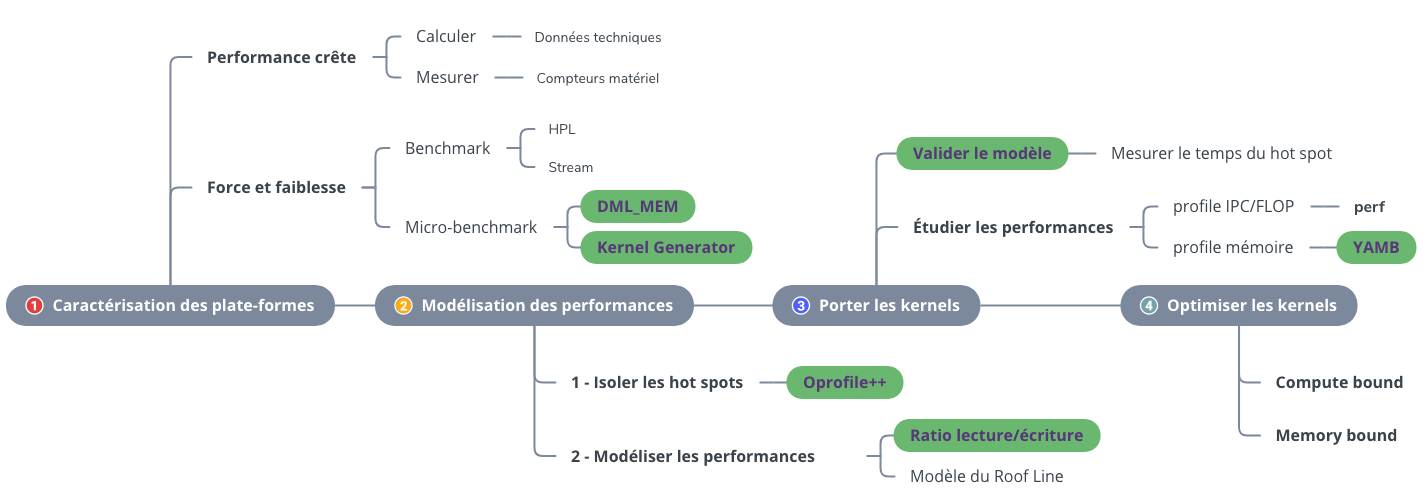
\includegraphics[width=17cm]{images/methodologie_step.png}
        \caption{\label{pic:methodologie_step_2} Méthodologie en 5 étapes pour caractériser et optimiser une application sur une nouvelle architecture.}
        \end{figure}
    
        Ce chapitre présente les cinq étapes de la méthodologie et suit la structure suivante:
        \begin{itemize}
            \item La \autoref{sec:methodo_step1} présente la première étape qui consiste à se tenir au courant de toutes les nouveautés technologiques ayant un potentiel pour être utilisées dans les centres de calculs. Nous discutons des caractéristiques clefs qu'il est nécessaire de quantifier pour estimer du potentiel de chaque architecture.
            \item La \autoref{sec:methodo_step2} discute des méthodes pour calculer ou mesurer la performance d'une architecture. Nous montrons comment deux des outils présentés dans le chapitre précédent peuvent être utilisés pour cela.
            \item La \autoref{sec:methodo_step3} s'intéresse aux applications et notamment à la modélisation de leur performance. Pour ce faire, nous présentons différents outils permettant d'isoler les \textit{hot spots} d'une application ainsi qu'un modèle de performance basé sur la performance du système mémoire.
            \item La \autoref{sec:methodo_step4} discute ensuite des principaux facteurs à étudier pour réaliser le choix des plateformes. 
            \item La \autoref{sec:methodo_step5} s'intéresse enfin au portage du code sur les plateformes sélectionnées précédemment. Nous y présentons une suite d'étape à suivre pour valider la bonne performance des noyaux et dans le cas contraire des étapes à suivre pour optimiser leur performance.
        \end{itemize}
        
        Pour les illustrer les différentes étapes, nous appliquons la méthodologie à l'étude des performances de la fonction \textit{triadd} (voir extrait de code \ref{lst:triadd}) du benchmark Stream \cite{McCalpin1995} sur un processeur Intel\textit{ Xeon Gold 6148} possédant 20 coeurs. Les matrices utilisées mesurent chacune 19.6 GB. 
        
\begin{lstlisting}[language=c,caption=Fonction Triadd extraite du benchmark Stream \ref{McCalpin1995},label={lst:triadd}, 
  basicstyle=\footnotesize, frame=tb,
  xleftmargin=.065\textwidth, xrightmargin=.065\textwidth]
for (j=0; j < STREAM_ARRAY_SIZE; j++)
    A[j] = B[j] + scalar * C[j];
\end{lstlisting}
